
The evaluation employs the SC-Math6 corpus, which consists of thousands of Chinese math problems. 
\dsviirl{} outperforms all Chinese LLMs, including both open-source and close-source models. 

\begin{table}[!ht]
    \centering
    \begin{tabular}{lccccc}
    \toprule
    \centering
    \textbf{Model Name} & \textbf{R Level} & \textbf{Comp. Score} & \textbf{Reas. Steps Score} & \textbf{OvrAcc Score} \\
    \midrule
    GPT-4-1106-Preview & \textbf{5} & 90.71 & 91.65 & 89.77 \\
    GPT-4 & \textbf{5} & 88.40 & 89.10 & 87.71 \\ \midrule
    \dsviirl{} & \textbf{5} & 83.35 & 85.73 & \textbf{84.54} \\
    Ernie-bot 4.0 & \textbf{5} & 85.60 & 86.82 & 84.38 \\
    Qwen-110B-Chat & \textbf{5} & 83.25 & 84.93 & 84.09 \\
    GLM-4 & \textbf{5} & 84.24 & 85.72 & 82.77 \\
    Xinghuo 3.5 & \textbf{5} & 83.73 & 85.37 & 82.09 \\
    Qwen-72B-Chat & \textbf{4} &78.42 & 80.07 & 79.25 \\
    ChatGLM-Turbo & \textbf{4} & 57.70 & 60.32 & 55.09 \\
    GPT-3.5-Turbo & \textbf{4} & 57.05 & 59.61 & 54.50 \\
    Qwen-14B-Chat & \textbf{4} & 53.12 & 55.99 & 50.26 \\
    ChatGLM3-6B & \textbf{3} & 40.90 & 44.20 & 37.60 \\
    Xinghuo 3.0 & \textbf{3} & 40.08 & 45.27 & 34.89 \\
    Baichuan2-13B-Chat & \textbf{3} & 39.40 & 42.63 & 36.18 \\
    Ernie-3.5-turbo & \textbf{2} & 25.19 & 27.70 & 22.67 \\
    Chinese-Alpaca2-13B & \textbf{2} & 20.55 & 22.52 & 18.58 \\
    \bottomrule
    \end{tabular}
    \caption{
    SC-Math6 Model Reasoning Level. 
    ``R Level'' stands for Reasoning Level, 
    ``Comp. Score'' stands for Comprehensive Score, 
    ``Reas. Steps Score'' stands for Reasoning Steps Score, 
    and ``OvrAcc Score'' stands for Overall Accuracy Score.
    }
    \label{tab:model_overall}
\end{table}

We further share more results in Figure~\ref{fig:code} on HumanEval and LiveCodeBench, where the questions of LiveCodeBench are selected from the period between September 1st, 2023, and April 1st, 2024.
As shown in the figure, \dsviirl{} demonstrates considerable proficiency in LiveCodeBench, achieving a Pass@1 score that even surpasses some giant models. 
This performance highlights the strong capability of \dsviirl{} in tackling live coding tasks. 

\begin{figure}[!ht]
    \centering
    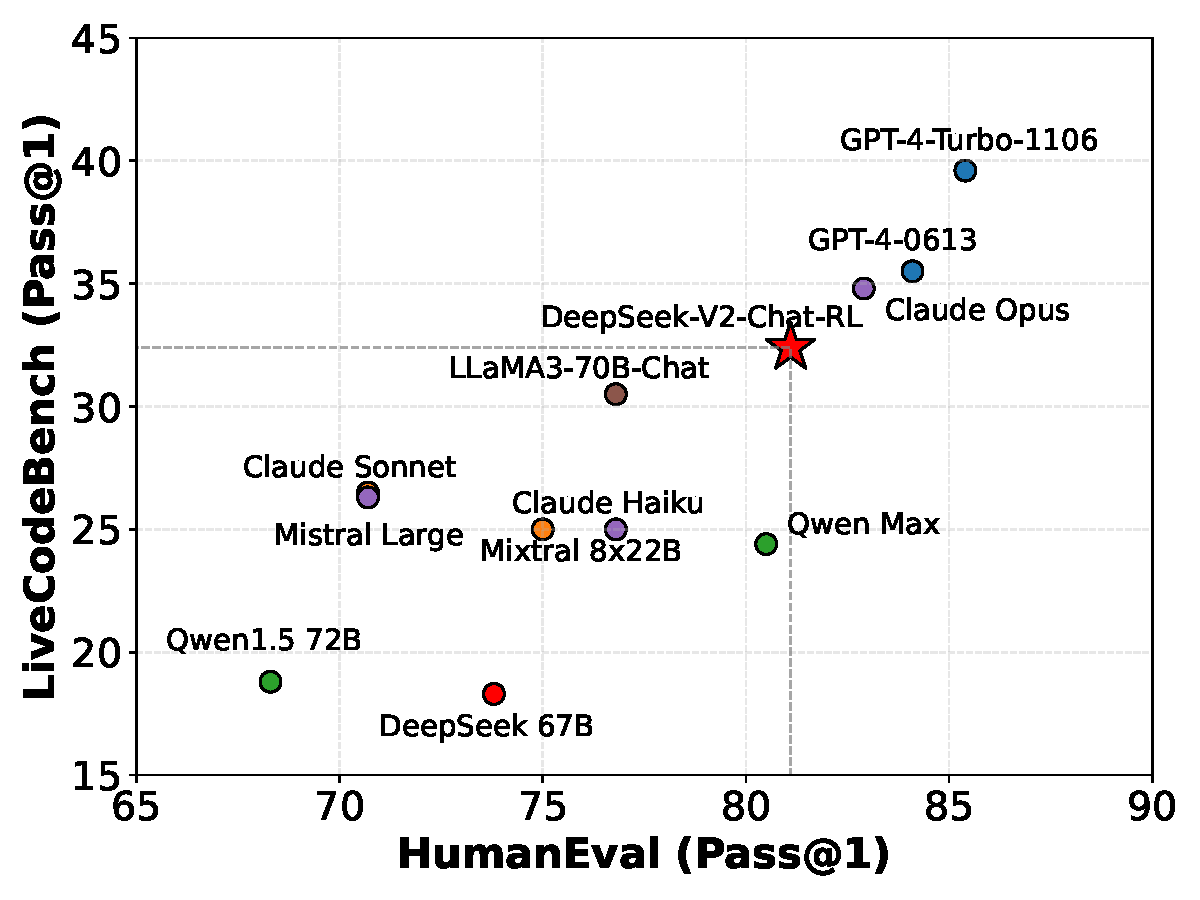
\includegraphics[width=0.8\linewidth]{figures/code.pdf}
    \caption{
    Evaluation results on HumanEval and LiveCodeBench. The questions of LiveCodeBench are selected from the period between September 1st, 2023 and April 1st, 2024.
    }
    \label{fig:code}
\end{figure}